\section{Experiments}
\label{sec:experiments}

\paragraph{Setup.} We code all 15,360 routed experts (46,080 matrices) of DeepSeek-V4.1-Flash, each at 3 bits per
weight. Calibration uses up to 65,536 routed rows per expert (seed 41) plus every attention-sink row, drawn from a
mixed web, code, math and multilingual corpus. Expert-level error is the NMSE of the expert output against the native
MXFP4 expert on up to 1,024 held-out routed tokens per expert. We aggregate it over the model as the ratio of mean
expert NMSE to EXL3's, with every expert weighted equally, and give the geometric mean of the per-expert ratios in
parentheses. The baseline is EXL3 at 3.0 bits per weight as published (exllamav3's own quantizer, rotation and
Hessian), fitted on the same calibration pool with the same seed and cap and measured on identical held-out rows.
Model-level metrics use 400 held-out 2,048-token windows (all 140 of the WikiText-2 test set and 260 from C4
validation), scored against the native model with llama.cpp's rule, which scores the second half of each window
without BOS (409,200 scored tokens). We report KL divergence, excess NLL of the true next token and top-1 agreement,
with paired bootstrap 95\% intervals over windows.

\paragraph{Damage and divergence.} Our evaluation runs the experts in FP16 arithmetic. With the \emph{native}
weights, this path alone has KL \final{F-KL} to the reference (top-1 \final{F-T1}) at an excess NLL of \final{F-NLL}.
Ulp-level differences swap near-tied top-$k$ routes, and the swaps propagate through later
layers~\citep{fu2025eaquant,park2026vsraq,gu2026routeflip}, but the change in mean NLL on these corpora is negligible.
Because KL also counts such route swaps, we take excess NLL as the measure of damage and KL as a measure of divergence,
and we compare KL only between models in the same arithmetic. GRAFT's decoded weights also run on the
reference's own expert kernels (\cref{sec:operands}). There the native weights reproduce the reference exactly, so
every difference comes from GRAFT's weights.

\begin{table*}[t]
\centering
\caption{DeepSeek-V4.1-Flash at 3 bits per weight (routed experts). Expert: held-out expert NMSE relative to EXL3 on
the same rows, ratio of means (geometric mean of ratios). Model level: 400 windows scored with the llama.cpp rule;
excess NLL of the true next token ($\Delta$NLL, nats), KL divergence and top-1 agreement against the native model,
with the experts in FP16 arithmetic except on the reference kernels. The second row is a control that runs the native
weights through the same FP16 arithmetic. Bits: stored bits per expert weight, all tensors
included.
$^\dagger$Ablation: per-matrix octave codebook instead of block flags (\cref{tab:ablation}).}
\label{tab:main}
\small
\setlength{\tabcolsep}{5pt}
\begin{tabular}{lccccc}
\toprule
 & bits & expert & $\Delta$NLL & KL & top-1\\
\midrule
native MXFP4 & 4.25 & -- & 0 & 0 & 100\%\\
\quad FP16 expert arithmetic & 4.25 & -- & \final{F-NLL} & \final{F-KL} & \final{F-T1}\\
EXL3 & 3.010 & 1.00 & \final{E-NLL} & \final{E-KL} & \final{E-T1}\\
\textbf{GRAFT} & 3.006 & \final{X-MEAN} (\final{X-GEO}) & \final{G-NLL} & \final{G-KL} & \final{G-T1}\\
\quad reference kernels & 3.006 & & \final{R-NLL} & \final{R-KL} & \final{R-T1}\\
octave codebook$^\dagger$ & 3.004 & \final{O-MEAN} (\final{O-GEO}) & \final{O-NLL} & \final{O-KL} & \final{O-T1}\\
\bottomrule
\end{tabular}
\end{table*}

\paragraph{Expert level.} Over the whole model, GRAFT's mean held-out expert error is \final{X-MEAN}$\times$ that of
EXL3 (geometric mean of the per-expert ratios \final{X-GEO}$\times$), and its error is lower on all but
\final{X-WORSE} of the \final{X-N} experts with held-out rows. The ratio is flat across depth (\final{X-LAYERS} per
layer; \cref{fig:layers}a). This is what the discrete-source argument predicts for a source whose grid structure is
the same in every layer. At 3 bits the memoryless reference is about \final{DS-BOUND3-1}$\times$ $D_G$, and GRAFT's
tile error is about \final{GRAFT-BOUND3} that reference. On tiles (\cref{fig:rd}b), where EXL3's codebook codes the
same \final{ROT-N} DeepSeek matrices after EXL3's rotation, the median over matrices of GRAFT's error relative to
EXL3's is \final{TILE-275} at 2.75 bits, \final{TILE-3} at 3, \final{TILE-325} at 3.25, \final{TILE-35} at 3.5 and \final{TILE-375} at 3.75.
The advantage thus grows with the rate, and at 4 bits GRAFT reproduces every sampled tile of \final{EXACT4} of the
matrices exactly.

\paragraph{Model level.} GRAFT's excess NLL is \final{G-NLL} nats against \final{E-NLL} for EXL3, a ratio of
\final{G-NLLR} (paired difference \final{G-DNLL-X}). Its KL is \final{G-KL} against \final{E-KL}, a ratio of
\final{G-KLR} (paired difference \final{G-DKL-X}), and its top-1 agreement is \final{G-T1} against \final{E-T1}. On
the reference's own kernels, GRAFT's KL is \final{R-KL}, slightly above that of the FP16 path (paired difference
\final{R-DKL-G}), and its excess NLL is \final{R-NLL}. Removing the arithmetic's own perturbation therefore does not
lower GRAFT's KL. This is consistent with the route swaps caused by the arithmetic overlapping those caused by the
weights rather than adding to them, although we did not trace individual routes to confirm the mechanism. Either
way, KL measured in one arithmetic cannot be split into an arithmetic part and a weight part by subtraction.

\begin{figure*}[t]
\centering
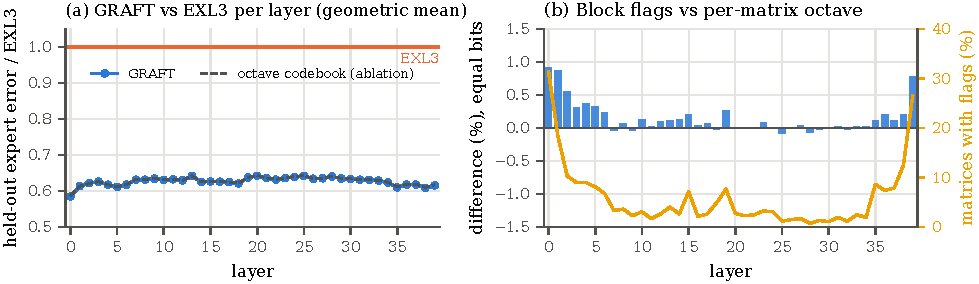
\includegraphics[width=\textwidth]{figures/fig_layers}
\caption{Held-out expert error per layer on DeepSeek-V4.1-Flash at 3 bits. (a) GRAFT and the octave-codebook ablation
relative to EXL3 on the same rows (geometric means; the two curves overlap). (b) Difference between GRAFT's error and
the octave codebook's at equal bits (bars), $100(\text{GRAFT}/\text{octave}-1)$, where zero means equal error, and
the share of matrices whose fit uses block flags (line).}
\label{fig:layers}
\end{figure*}

\paragraph{Ablations.} \Cref{tab:ablation} quantifies GRAFT's design choices. Every row is fitted on the same
calibration rows and measured on the same held-out rows. Where an ablation spends a different number of bits, we
compare at equal bits using the measured held-out rate curve of the octave-codebook fit, which gives an error factor
of \final{RHO} per extra quarter bit at 3 bits (14 experts).
\begin{itemize}[leftmargin=1.1em,itemsep=1pt,topsep=2pt]
\item \emph{The code or the fitting objective.} GRAFT's fit differs from EXL3's in the objective (gated,
token-weighted $H$ and column weights, shrinkage, down-projection statistics from the quantized gate/up activations)
as well as in the code. An EXL3 refit with GRAFT's objective on the same calibration rows has \final{ATTR-OBJ} the
held-out error of EXL3 as published (geometric mean \final{ATTR-OBJ-GEO}, \final{ATTR-N} experts). GRAFT has
\final{ATTR-G} the error of this refit (geometric mean \final{ATTR-G-GEO}) and is lower on all but
\final{ATTR-G-WORSE} experts, so the objective accounts for a few percent and the grid-aligned code for the rest.
\item \emph{Block flags or a per-matrix octave codebook.} Instead of using flags, a matrix can move a fraction of its
trellis states one octave down, so that states whose top bits are set decode at half value. The two approaches reach
the same error. Over all \final{X-N} experts, the octave codebook has \final{O-RAW} GRAFT's held-out error at GRAFT's
bits and \final{O-EQ} at equal bits. The two are within $\pm$0.3\% in \final{O-LAYERS-N} of
40 layers and at most \final{O-LAYERS-MAX} apart in the first and last layers (\cref{fig:layers}b). The model-level KL
of the octave codebook is \final{O-KL}, against \final{G-KL} for GRAFT (difference \final{G-DKL-O}). Flags are needed
on \final{FLAG-SHARE} of the matrices and the octave on \final{OCT-SHARE}, and only flags keep the decoded blocks
MXFP4. On fit tiles at 3.5 bits the flags are ahead, with \final{FLAGS35} the octave codebook's error on
\final{FLAGS35-N} matrices.
\item \emph{Flags off.} On the \final{FLAGSOFF-N} flagged experts of the last layer, removing the flags raises
held-out error by only \final{FLAGSOFF-PCT} at equal bits, so at 3 bits the flags roughly break even on error. Their
benefit is that they keep the decoded blocks MXFP4. They also decode in fewer instructions than
the octave codebook (\final{K-B200-ON} against \final{K-B200-OCT} per weight on B200), and at 3.5 bits they are ahead
(above).
\item \emph{Rate allocation.} Moving bits between matrices according to their predicted contribution to expert
error, at the same stored size, lowers mean expert error by \final{ALLOC-ERR} (octave codebook, all experts) but KL
by only \final{ALLOC-KL}. It also lowers top-1 agreement (\final{ALLOC-T1} vs \final{FLAT-T1}) and raises excess NLL
(\final{ALLOC-NLL} vs \final{FLAT-NLL} on 40 windows, too few to resolve the difference). Allocation by our
expert-error estimator therefore did not improve model-level quality in this experiment, and GRAFT codes every
matrix at the same rate.
\item \emph{The trellis or a 3-bit scalar code.} Scalar 3-bit codebooks of 8 values per 8 columns, fitted with the
same objective and error feedback, have \final{SCALAR-EF} GRAFT's held-out error at the same bits (\final{SCALAR-N}
experts in \final{SCALAR-LAYERS} layers). With plain rounding they have \final{SCALAR-RTN}, and with an MX block
scale per 32 weights at \final{SCALAR-MX-BPW} bits they still have \final{SCALAR-MX}. An 8-value table can hold at
most 8 of the source's 15 levels, whereas the fitted trellis reproduces about \final{EXACT} of the source weights
exactly (within 5\% of a grid step after the column scale, on octave-codebook fits of 20 experts at 3 bits).
\end{itemize}

\begin{table}[t]
\centering
\caption{Ablations: error relative to GRAFT (equal bits unless marked). Top: measured held-out expert error on the
experts listed. Bottom: predictions of the selection estimator, not held-out measurements, given as the typical
(geometric-mean) and total fit-weighted tile error of the octave-codebook fits over \final{KNOB-N} matrices.}
\label{tab:ablation}
\footnotesize
\setlength{\tabcolsep}{2pt}
\begin{tabular}{@{}llr@{}}
\toprule
change & measured on & error\\
\midrule
EXL3 code, GRAFT's objective & all experts & \final{ATTR-INV}\\
octave codebook instead of flags & all experts & \final{O-EQ}\\
no block flags & \final{FLAGSOFF-N} experts, L39 & \final{FLAGSOFF}\\
3-bit scalar tables, error feedback & \final{SCALAR-N} experts & \final{SCALAR-EF}\\
\quad plain rounding & \final{SCALAR-N} experts & \final{SCALAR-RTN}\\
\quad + MX scales (\final{SCALAR-MX-BPW} bits) & \final{SCALAR-N} experts & \final{SCALAR-MX}\\
free (non-pow.-two) column scales & earlier code, 2 layers & $+$\final{FREE-SCALES}\\
\midrule
tail band fixed at $d=0$ & estimator & \final{KNOB-BAND-GEO} / \final{KNOB-BAND-TOT}\\
no group multipliers & estimator & \final{KNOB-MULT-GEO} / \final{KNOB-MULT-TOT}\\
\bottomrule
\end{tabular}
\end{table}
